\section{Обработка сигнала с детектора}\label{sec:secSignalProcessing}

Экспериментальная установка в физике высоких энергий или физике тяжёлых ионов ставит своей задачей восстанавливать события, произошедшие в области первичного взаимодействия. Такой областью будет являться точка взаимодействия пучка с мишенью в случае эксперимента с фиксированной мишенью, либо точка взаимодействия встречных пучков на коллайдерном эксперименте. Для выполнения этой задачи в некоторой области рядом с точкой взаимодействия ставят набор из нескольких детекторов, регистрирующих вторичные частицы и их продукты распада. Детекторы вырабатывают электрические сигналы, которые в случае современного крупного эксперимента необходимо доставить в ЭВМ, чтобы выполнять программную обработку, включающую в себя реконструкцию треков и частиц и анализ многочисленных распределений.

%В зависимости от исследуемой физики, детекторы могут охватывать различные геометрические направления. Есть две типичные конфигурации. В первой --- детекторы имеют форму цилиндров, охватывающих точку взаимодействия, во второй - детекторы образуют плоскости, расположенные друг за другом. Обычно бочка используется на коллайдере, а плоские слои на фиксированной мишени. CBM --- это второй случай. Но есть и исключения, например, установка LHCb, имеющая структуру плоских слоёв, установленных на коллайдере.

В этой главе обсуждаются решения, выбранные CBM для организации считывания данных с детекторной установки.

\textbf{Задача: дать общую картину --- детектор, передняя электроника, передающая электроника, ЭВМ. Затем указать, что вот типа электроника с внешним триггером, а вот самотриггирующаяся электроника. Далее переходим к free-running DAQ.}

Рассмотрим общую последовательность обработки сигнала детектора частиц.
% Разные типы детектирующих приборов
Источником является некоторое детектирующее устройство (или просто детектор). В зависимости от типа детектируемых частиц и внешних условий --- радиационная среда, температура, частота регистрации --- это может быть фотодиод, фотоэлектронный умножитель (ФЭУ), полупроводниковый детектор, микроканальная пластина, газовый электронный умножитель, и т.д. Все эти детекторы обладают таким общим свойством, что выходной сигнал, несущий информацию о зарегистрированной частице, это относительно слабый токовый импульс. В любом случае, для того, чтобы выполнять дальнейшую обработку этого сигнала в ЭВМ его необходимо оцифровать.

% Общие слова об обрабатывающей электронике
В связи с этим обрабатывающую электронику условно можно разделить на переднюю и остальную. Основная задача передней электроники --- оцифровать выходной аналоговый сигнал детектирующего устройства, при необходимости предварительно его усилив и отфильтровав. Передача аналогового сигнала затруднена, поэтому его обработка и оцифровка обычно выполняется как можно ближе к месту, где этот сигнал вырабатывается, т.е. непосредственно на детекторе. В простом случае последующие слои электроники концентрируют и передают оцифрованные сигналы со многих каналов передней электроники. В более сложном случае возможна какая-то аппаратная обработка оцифрованных сигналов, например архивация или фильтрация с целью уменьшения потока данных.

% Разные способы оцифровать сигнал
Разработан целый ряд подходов к оцифровке сигналов с детекторов. Каждый из них лучше всего подходит к определённому детектору, однако возможно применение методов, разработанных для одного детектора, для оцифровки сигналов с другого детектора. Перечислим лишь некоторые из них. Если не вдаваться в подробности реализации, можно выделить следующие способы: регистрация момента времени прихода фронта, регистрация амплитуды сигнала, непрерывное семплирование (ещё\todo). Практически всегда требуется регистрация момента времени прихода сигнала, поэтому широко применяются комбинации перечисленных способов --- регистрация амплитуды сигнала вместе с моментом времени прихода переднего фронта, регистрация моментов времени переднего и заднего фронтов без захвата амплитуды, регистрация момента времени переднего фронта и формирование ограниченного числа семплов после него.

% Предусилитель/шейпер, фильтр
Если необходимо предварительное усиление, то применяют один из двух типов усилителей --- зарядочувствительный усилитель либо \todo. В силу устройства зарядочувствительный усилитель является также формирователем (шейпером). Любая электроника подвержена шумам, поэтому для подавления шумов сигнал обычно предварительно проходит фильтр нижних частот, эффективно отрезающий частоты выше некоторого значения. (Что-то сказать про шейпирование и его неизбежность и влияние на временные характеристики) Ещё один способ борьбы с шумами --- фильтрация по амплитуде, т.е. установление некоторого порога по напряжению, ниже которого сигнал игнорируется. 

% Реализация
Описанные процедуры обработки сигнала могут быть реализованы на разной аппаратной платформе. Самый примитивный вариант --- это когда канал реализуется с применением ``сквозного монтажа'' (THT) или ``поверхностного монтажа'' (SMT, SMD) \todo таких-то компонентов. В принципе, это возможно, но в этом случае геометрические размеры определяют заметное время прохождения сигнала, таким образом ограничивая частоту функционирования. Также габариты ограничивают плотность каналов в пространстве и, вообще говоря, стоимость такой электроники выше современных компактных вариантов. В эксперименте CBM ожидается огромное число каналов при очень высокой плотности в пространстве. Один только детектор RICH будет иметь более 60000 каналов при плотности каналов около $0.5$ см$^{2}/$канал. Следовательно, рассматриваются более продвинутые технологии --- интегральные схемы, в том числе программируемые.

% ASIC vs. FPGA
На данный момент существует множество разновидностей интегральных схем, однако наибольший интерес в CBM (экспериментальной физике\todo) проявляется к интегральным схемам специального назначения (ASIC) и программируемым пользователем вентильным матрицам (ППВМ, FPGA). ASIC уже широко применяются в экспериментальной физике и в быту на протяжении десятилетий, в то время как ППВМ доступны сравнительно недавно. Эти два варианта принципиально отличаются тем, что ASIC невозможно изменить после изготовления, а FPGA не имеет какой-либо программы по умолчанию и программируется пользователем. Более того, программа FPGA стирается при отключении питания, поэтому рядом необходимо обеспечить постоянную память, из которой FPGA берёт программу при загрузке. Процесс проектирования FPGA фактически заключается в процессе разработки прошивки на языке описания аппаратуры (HLD, verilog), при этом в любой момент есть возможность применить прошивку к чипу чтобы выполнить отладку. Достоинство ASIC заключается в том, что чипы изготавливаются относительно дёшево при большом размере партии. Высокую стоимость имеет шаблон, на основе которого можно дёшево изготовить большую партию чипов. С другой стороны процесс проектирования ASIC осложнён тем, что если для отладки требуется физический экземпляр, а не программная модель, то требуется изготовление шаблона.

% Дискриминатор
Рассмотрим схему, когда аналоговый импульс с детектора обрабатывается электроникой, регистрирующей момент времени прихода переднего фронта. Любой сигнал переключается за некоторое ненулевое время, поэтому необходимо определить точку, обозначающую фронт. Для этого применяют дискриминатор --- прибор, вырабатывающий логический ``0'', когда входной сигнал ниже установленного порога, и логическую ``1'', когда входной сигнал выше установленного порога. Таким образом точка пересечения сигнала и порога это точка, условно обозначающая момент времени прихода сигнала. На выходе дискриминатора получается логический сигнал, который необходимо преобразовать в цифровой с помощью время-цифрового преобразователя (ВЦП). На выходе ВЦП уже будет цифровой сигнал, а не логический.
%Далее могут работать концентраторы данных и какие-то ещё платы, обеспечивающие приём данных в ЭВМ. Таким принимающим устройством может быть обычный сетевой интерфейс, работающий с Ethernet. В CBM это не так, поэтому нужен FLIB.

% Заключение - разработки чипов в CBM
Коллаборацией CBM ведётся разработка нескольких чипов, на базе которых будут построены платы передней электроники. STS-XYTER --- ASIC для кремниевой трековой системы, регистрирующий амплитуду сигнала и временную отметку переднего фронта. SPADIC --- ASIC для детектора переходного излучения, имеющий богатый функционал, но, самое главное, выполняющий непрерывное семплирование входного сигнала. (\textbf{Наверное, нет смысла описывать подробнее --- слишком сложный чип}) Группы CBM RICH, HADES RICH и PANDA DIRC совместно занимаются разработкой программ для FPGA, выполняющих функции дискриминатора и ВЦП.

% Аппаратный триггер
(Тут нужно обсудить и почитать ещё. Возможен ли такой сценарий, в наше время или в прошлом, когда триггер чисто аналоговый. То есть передняя электроника игнорирует сигнал до тех пор, пока не сработает схема совпадения с триггером. В той модели традиционного триггера, которую я себе сейчас представляю, входной сигнал обрабатывается непрерывно, но выпускается на выход из буфера только при наличии триггера. Вероятно, возможно и то и то, но вопрос в том, что реально используется, что более распространено.)
Рассмотрим систему считывания и сбора данных ``традиционного'' эксперимента, имеющего аппаратный триггер. Каждый канал передней электроники имеет выходной буфер, куда по принципу FIFO складываются оцифрованные входные сигналы. В экспериментальной установке присутствуют детекторы, вырабатывающие триггер --- сигнал, который заводится (условно) на каждый канал считывания, и говорит о том, что произошло интересное событие, которое необходимо сохранить для последующей обработки. Данный подход имеет свои причины. Во-первых, до недавнего времени физические эксперименты не требовали высоких частот регистрации --- выполнение физической программы при относительно низких частотах первичного взаимодействия было осуществимо в разумные сроки. Во-вторых, многие регистрирующие приборы имеют заметное ``мёртвое время'' --- время после регистрации одного входного сигнала, в течение которого прибор не может обрабатывать последующие входные сигналы. Следовательно, если канал регистрирует ложный входной сигнал, велика вероятности того, что будет пропущен полезный сигнал. С развитием электроники ``мёртвое время'' уменьшалось. Более того, возможность применения принципиально другой считывающей электроники, как например чисто временной канал, реализованный в ППВМ, для обработки сигналов с МА~ФЭУ в CBM~RICH, исследуемая в данной работе, позволяет на порядки снизить ``мёртвое время'' и повысить точность регистрации временной отметки в ущерб полноты информации.

(Сюда подмешивается секция 2.2 \todo)

% Программный триггер
В CBM планируется использование программного триггера. Это означает, что для того, чтобы принять решение, сохранять принятые данные или нет, необходимо выполнить полную реконструкцию события, включая реконструкцию треков, которая является высоко-затратной задачей. Рассматривается также возможность на определённых этапах работы установки использовать для выработки триггера частичную реконструкцию. Например исследуется возможность триггирования по результатам реконструкций треков только в MUCH, когда стоит задача поиска (\todo такой-то частицы).

В ``традиционном'' эксперименте триггер может формироваться в результате логических операций над сигналами с нескольких детекторов, реализованных аппаратно. Такая логика работает за (\todo масштаб времени). Реконструкция треков выполняется за гораздо большее время (\todo на столько-то порядков выше). По этой причине необходимо иметь не только буфер в электронике --- его будет недостаточно. 

(Сказать о том, что нужно хорошо настраивать пороги.)

\subsection{Система считывания и сбора данных эксперимента CBM}\label{CBMreadout}

Блок-схема архитектуры системы считывания и сбора данных эксперимента CBM приведена на \figref{fig:CBMreadout}.

\begin{figure}[H]
\centering
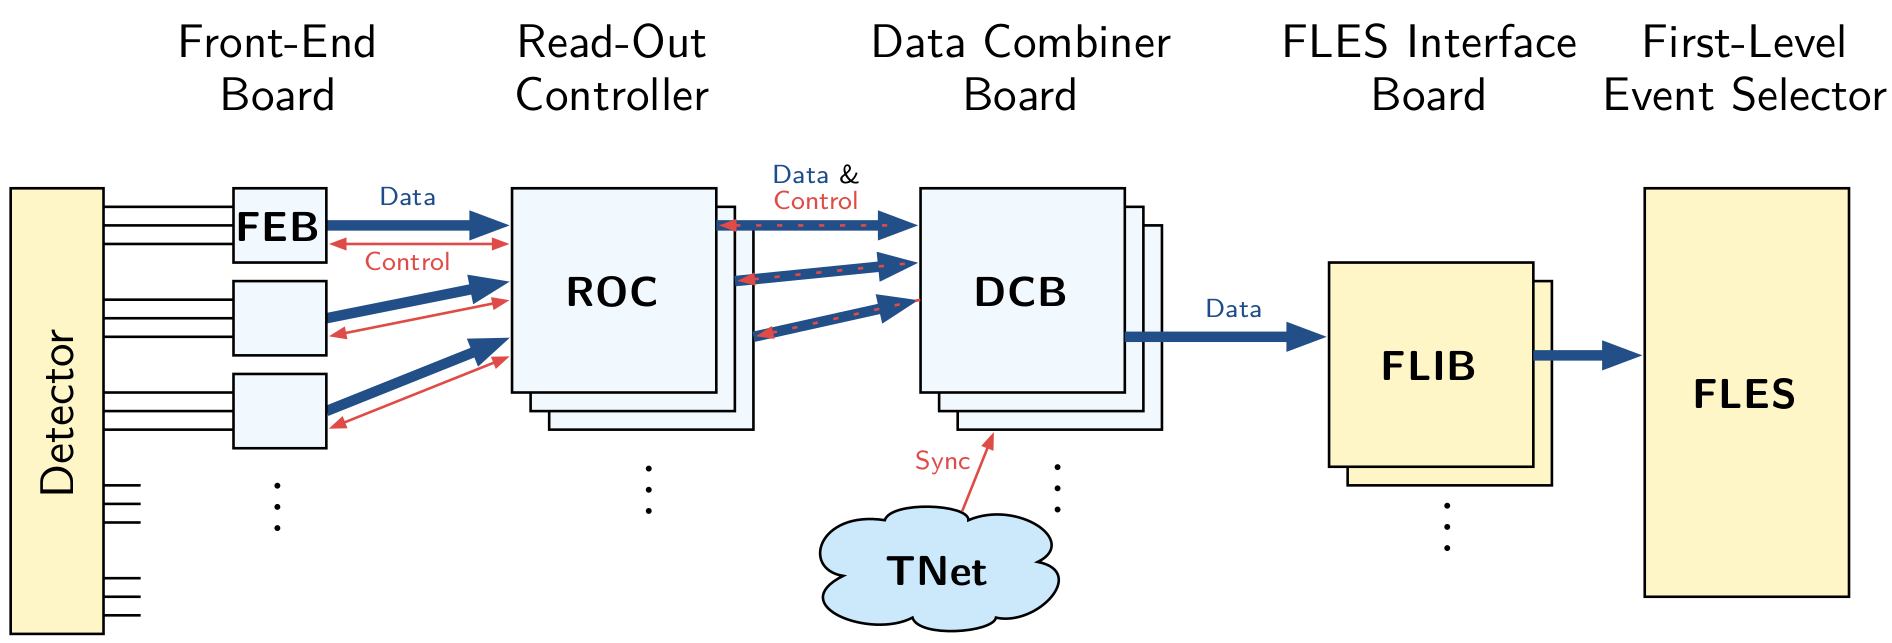
\includegraphics[width=0.7\textwidth]{pictures/CBMreadout.png}
\caption{Система считывания и сбора данных CBM.}
\label{fig:CBMreadout}
\end{figure}

\textbf{Развёрнутое описание выше делается для понимания этой секции.}

Источником электрических сигналов являются детекторы, выполненные по разным технологиям, и требующие оцифровки различными способами. Эта оцифровка выполняется разнообразными платами передней электроники (FEB), имеющими разные принципы и основанными на различных чипах. Затем цифровые данные опрашиваются с плат передней электроники контроллерами считывания (ROC). После этого данные группируются в соответствующих платах (DCB) и поступают во FLES через платы FLIB.

\subsection{FLES}\label{sec:secFLES}

\textbf{переработать}
Всё вместе привело к разработке аппаратно-программного комплекса, называемого системой отбора первого уровня --- First Level Event Selector (FLES). По сути DAQ-часть (приём данных) неотделима от FLES, поэтому иногда эту систему называют FLES/DAQ.
Отличительные черты FLES --- самотриггирующаяся электроника, несколько уровней концентрации данных, многочисленные буферы, формирование срезов времени, построение интервалов и только после этого мы переходим к построению событий.

% 1 - Приём данных и формирование срезов времени
Функционал FLES/DAQ можно разбить на три части. Первая --- приём и объединение данных, поступающих с группы каналов, в срезы времени (timeslice). Такую группу образует некоторое множество каналов одного детектора, количество которых определяется ожидаемым потоком данных, а ограничение диктуется максимальной пропускной способностью входного канала FLES.

% 2- Interval building
Один из наиболее важных и нестандартных этапов работы FLES --- это построение интервалов (Interval building, IB). Построение интервалов --- это получение контейнеров с данными со всех детекторов за некоторый интервал времени путём перегруппировки данных из срезов времени. Суть построения интервалов показана на \figref{fig:IntervalBuilding}. Данные от одного ``входного узла'' (input node, IN) приходят от группы каналов какого-то детектора и представляет собой последовательность срезов времени. Задача заключается в том, чтобы объединить все срезы, соответствующие одному интервалу времени, чтобы дальше передать на ``вычислительный узел'' (processing node, computing node, CN).

\begin{figure}[H]
\centering
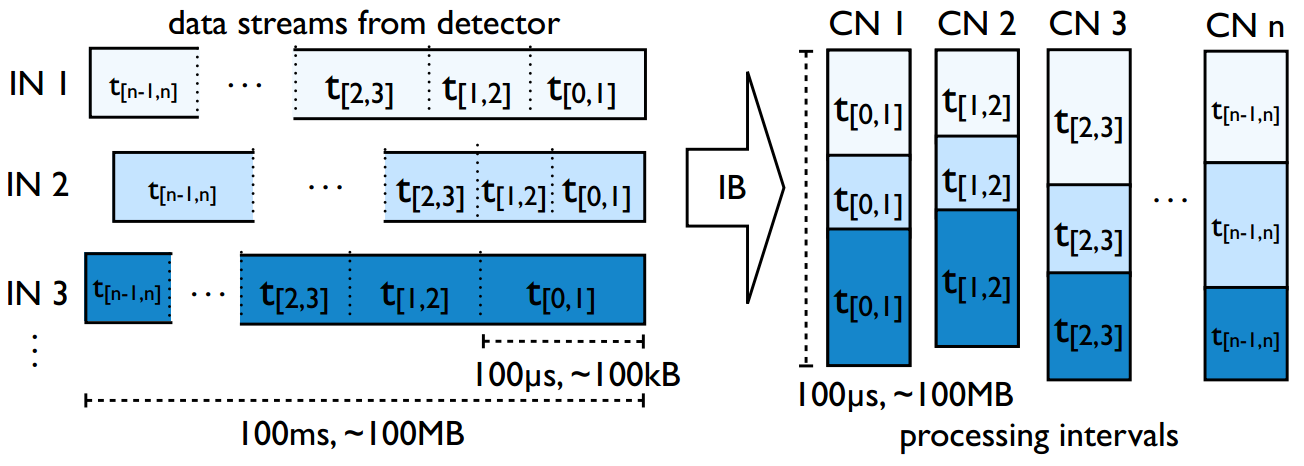
\includegraphics[width=0.7\textwidth]{pictures/Interval_building.png}
\caption{Построение интервала.}
\label{fig:IntervalBuilding}
\end{figure}

% 3- Этап после построения интервалов
Заключительный этап обработки данных во FLES --- восстановление событий в интервале, реконструкция треков и частиц в восстановленных событиях и выработка сигнала о сохранении или отбросе интервала.

% Численные оценки, определение FLES как сети из узлов
Для эксперимента CBM был выполнен оценочный расчёт. Отправная точка --- возможно сохранение 1~Гбайт/сек данных. Считается, что одно событие CBM в среднем имеет объём 40~Кбайт. Отсюда следует, что максимальная частота первичного взаимодействия может быть 25~кГц. В стартовой конфигурации CBM частота первичного взаимодействия равна 10~МГц, следовательно, необходимо уменьшить поток данных в 400~раз. В полноценном режиме работы CBM ожидается 25~МГц, т.е. $ 25 \cdot 10^{6} \cdot 40 $ Кбайт = 1 Тбайт/сек. Планируется разбить этот поток в 1~Тбайт/сек на 1000 входных каналов FLES, каждый по 1~Гбайт/сек, передающихся по 10-Гбитным оптическим каналам связи. Один входной канал FLES соответствует одному ``входному узлу'' --- ЭВМ с установленной платой FLIB. Все вычисления, необходимые для отбора данных будут осуществляться на так называемых ``вычислительных узлах''. Входные и вычислительные узлы объединены в компьютерную сеть посредством InfiniBand QDR, образуя уникальную распределённую вычислительную систему, называемую FLES, см. \figref{fig:FLESarch}. Вычислительная подсеть будет иметь приблизительно 60000 ядер.

\begin{figure}[H]
\centering
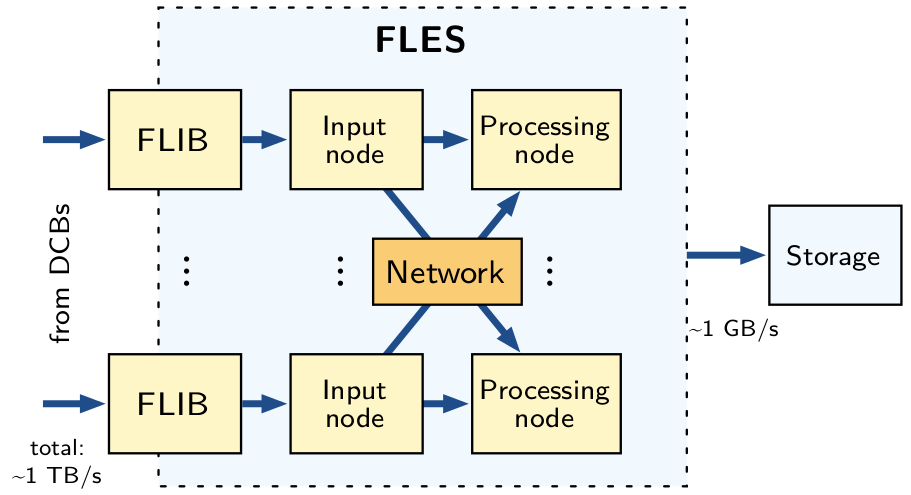
\includegraphics[width=0.7\textwidth]{pictures/FLESarch.png}
\caption{Общая схема устройства FLES.}
\label{fig:FLESarch}
\end{figure}

% Реконструкция по одному детектору
Планируется также, что FLES сможет функционировать в особом режиме, когда для выполнения реконструкции с целью отбора данных для сохранения будет использоваться только часть входного потока. На \figref{fig:PartialIB} приведена блок-схема функционирования FLES в таком режиме. Это имеет смысл при работе эксперимента над некоторыми пунктами физической программы, но принципиальная возможность и эффективность реконструкции частиц с целью триггирования по ограниченному набору детекторов является предметом исследований. Например, можно восстанавливать \todo такую-то частицу только по трекам в MUCH. При этом система приёма данных работает в полную силу --- идёт приём со всех детекторов и никакие данные не выбрасываются до тех пор, пока не будет выполнена реконструкция по данным с MUCH. Если в результате реконструкции выясняется, что принятая порция данных потенциально интересна, то она извлекается из буферов и записывается. Это позволяет \todo снизить поток сохраняемых данных в \todo раз, что особенно актуально при экстремально высоких частотах взаимодействия.

\begin{figure}[H]
\centering
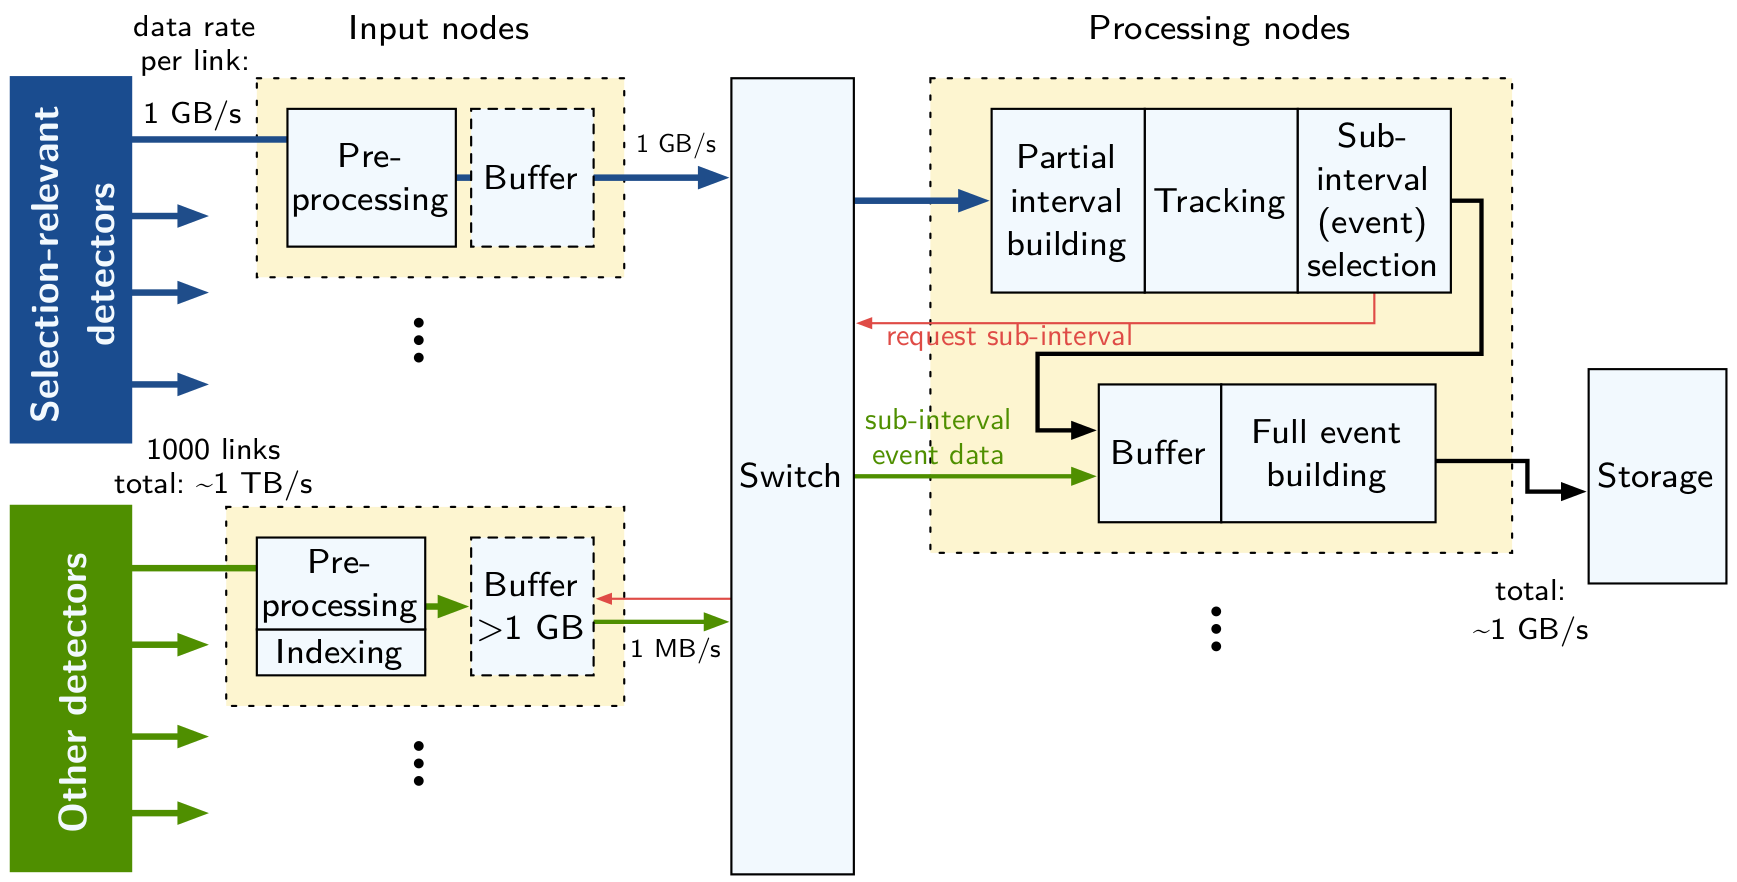
\includegraphics[width=1.0\textwidth]{pictures/PartialIB.png}
\caption{Блок-схема функционирования FLES в режиме отбора по данным с части детекторов.}
\label{fig:PartialIB}
\end{figure}

\todo Подробное описание того, что на картинке

% FLIB
\subsubsection{FLES Interface Board}\label{sec:FLIB}

В качестве платы-интейфейса между электроникой, разрабатываемой специально для CBM, и ЭВМ стандартной архитектуры, будет выступать плата, в общем называемая платой интерфейса FLES --- FLES Interface Board, или FLIB. FLIB можно рассматривать как особый сетевой интерфейс, основной задачей которого является предоставление данных, поступающих по входным каналам, центральному процессору ЭВМ. В отличие от сетевого интерфейса Ethernet, данные поступают от разнородных плат передней электроники по разным протоколам. В качестве платформы для реализации FLIB в CBM рассматривается коммерческая PCI-E плата HTG~K-7. Архитектура FLIB показана на \figref{fig:FLIBarch}. Основные компоненты FLIB --- драйверы входных оптических портов, программируемая пользователем вентильная матрица (ППВМ, FPGA), оперативное запоминающее устройство (ОЗУ) и драйвер шины PCI-Express. 

\begin{figure}[H]
\centering
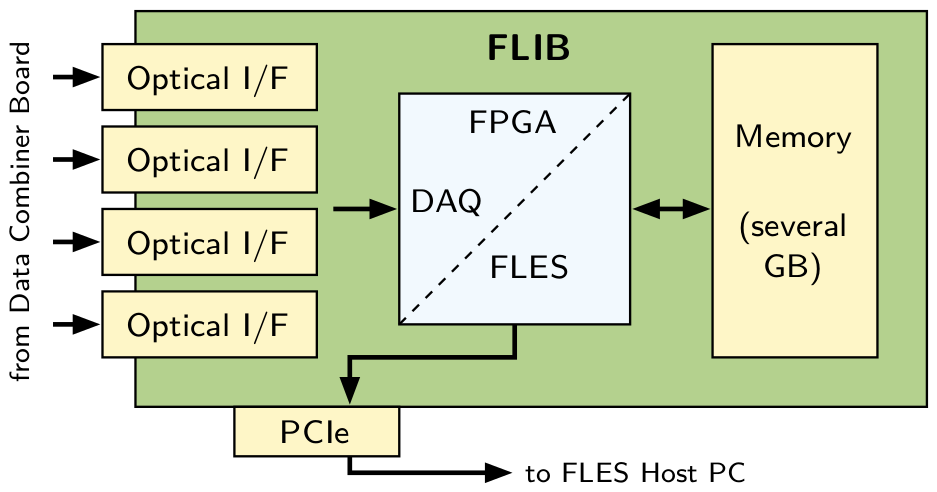
\includegraphics[width=1.0\textwidth]{pictures/FLIBarch.png}
\caption{Архитектура FLIB.}
\label{fig:FLIBarch}
\end{figure}